%! Author = gramic
%! Date = 19.03.24

% Preamble
\begin{flushleft}
    \subsubsection{Sharding}
    \paragraph{Vertikales / Horizontales Sharding}
    Tabellen können horizontal oder vertikal partitioniert werden.
    Bei der vertikalen Partitionierung werden Tabellen ähnlich zur Normalisierung vertikal aufgeteilt, nur dass der Primary Key derselbe bleibt.
    Nachfolgend ein Beispiel zur vertikalen Partitionierung:
    \begin{figure}[H]
        \centering
        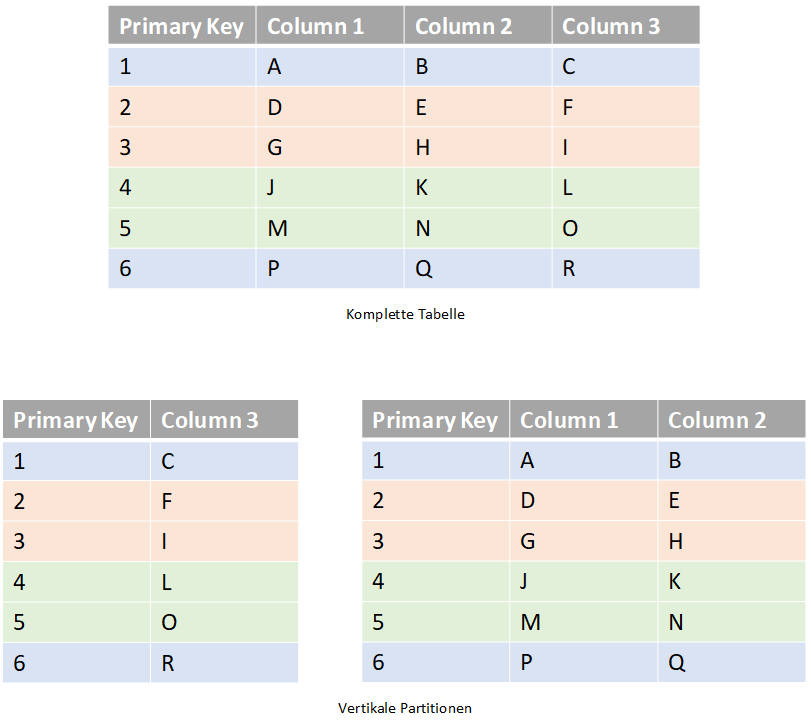
\includegraphics[width=0.8\linewidth]{source/implementation/evaluation/excursus_architecture/sharding_vertical_partitioning}
        \caption{Sharding - Vertikale Partitionierung}
        \label{fig:sharding_vertical_partitioning}
    \end{figure}
    \clearpage
    Die horizontale Partitionierung geht den umgekehrten Weg.
    Die Datensätze einer Tabelle werden anhand bestimmter Regeln in Partitionen mit gleicher Struktur verteilt.
    Nachfolgend ein Beispiel einer horizontalen Partitionierung:
    \begin{figure}[H]
        \centering
        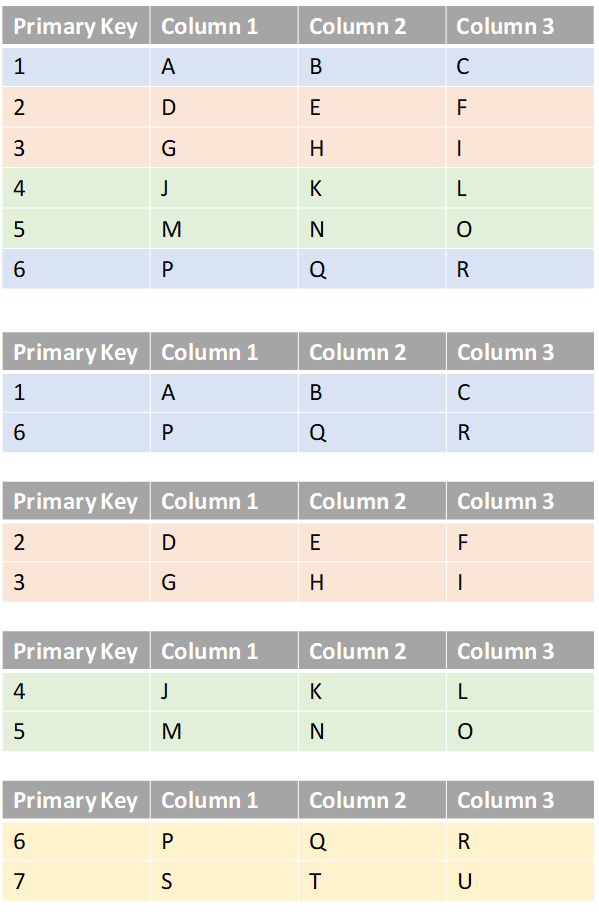
\includegraphics[width=0.8\linewidth]{source/implementation/evaluation/excursus_architecture/sharding_horizontal_partitioning}
        \caption{Sharding - Horizontales Partitionierung}
        \label{fig:sharding_horizontal_partitioning}
    \end{figure}
    Horizontales Partitionieren wird oft für das Sharding von Tabellen benutzt.
    Die Partitionen entsprechen dann den Shards.
\begin{flushleft}
\end{flushleft}
    \paragraph{Key Based Sharding}
    Hierbei wird das Sharding anhand eines oder mehreren Keys ausgeführt.
\begin{flushleft}
\end{flushleft}
    \paragraph{Range Based Sharding}
    Das Sharding wird dabei anhand von Ranges ausgeführt.
    Zum Beispiel anhand von Preis-Ranges.
\begin{flushleft}
\end{flushleft}
    \paragraph{Directory Based Sharding}
    Hierfür wird eine Lookup-Tabelle geführt, welche die Schlüssel für das Sharding bereitstellen.
    Anhand dieser werden dann die entsprechenden Zieltabellen aufgeteilt.
\begin{flushleft}
\end{flushleft}
    \paragraph{Hash Based Sharding}
    Das Hash Based Sharding ist eine Form des Range Based Shardings, bei dem Hashwerte der Datensätze benutzt werden.
    Je nach Bereich wird der Datensatz dann einem Shard zugewiesen.
\end{flushleft}